\documentclass[letterpaper,10pt]{book}
% Change to 10 pt
\usepackage{pdfpages}
\usepackage{morewrites}			% to counteract the no write space problem
\setcounter{tocdepth}{6}

\usepackage[framemethod=TikZ]{mdframed}

\usepackage{fancyhdr}

\usepackage{paralist}
\usepackage{amsmath}
\usepackage{amsfonts}
\usepackage{amssymb}
\usepackage{graphicx}

\usepackage{datetime}
%\usepackage{ulem}

%\usepackage[nottoc]{toobibind}

\usepackage[inline]{enumitem}

% Outer margin at 2.50 is exacty correct to fit the ``corruption alert'' tables
\usepackage[inner=1.0in, outer=2.50in, top=2.54cm,bottom=2.54cm, marginparwidth=2.25in]{geometry}

\usepackage{marginnote}
\usepackage{longtable}
\usepackage{booktabs}
\usepackage{xcolor}

\usepackage{soul}

%%%%%%%%%%%%
\definecolor{ForestGreen}{rgb}{0.00,0.29,0.098}
%%%%%%%%%%%%

\usepackage{marginnote}

\usepackage{imakeidx} 
\usepackage[
	backref=true,
	style=numeric,
%	citestyle=numeric,
	backend=bibtex
	]{biblatex}
\usepackage[driverfallback=hypertex,colorlinks=True]{hyperref}
\usepackage{cleveref}

\makeindex[name=scripture,columnsep=20pt, columnseprule=True,columns=3, title=Scripture References]
\makeindex[name=speaker,columnsep=20pt, columnseprule=True,,columns=2, title=Sermon Creator]
\makeindex[name=series,columnsep=20pt, columnseprule=True,,columns=2, title=Sermon Series]
\makeindex[name=date,columnsep=20pt, columnseprule=True,columns=2, title=Sermon Date]
\makeindex[name=event,columnsep=20pt, columnseprule=True,columns=2, title=Event]
\makeindex[name=topic,columnsep=20pt, columnseprule=True,columns=2, title=Topic]
\makeindex[name=AWIP,columnsep=20pt, columnseprule=True,columns=3, title=All Words in Passage]
\makeindex[name=NWIV,columnsep=20pt, columnseprule=True,columns=3, title=Number of Words in Verse]
\makeindex[name=PNIP,columnsep=20pt, columnseprule=True,columns=3, title=Proper Names in Passage]
\makeindex[name=PEIP,columnsep=20pt, columnseprule=True,columns=2, title=Prophetic Events in Passage]
\makeindex[name=TWPAQ,columnsep=20pt, columnseprule=True,columns=1, title=13-Word Phrases and Quotes]
\makeindex[name=PFTTIS,columnsep=20pt, columnseprule=False,columns=3, title=Phrases found 13 times in scripture]
\makeindex[name=WFTTIS,columnsep=20pt, columnseprule=False,columns=3, title=Words found 13 times in scripture]
\makeindex[name=WFITV,columnsep=20pt, columnseprule=False,columns=3, title=Words found in exactly 13 verses]
\makeindex[name=EVENTS,columnsep=20pt, columnseprule=False,columns=2, title=Sermon Log by Place]
\makeindex[name=QUESTIONS,columnsep=20pt, columnseprule=False,columns=2, title=Bible Questions]
\makeindex[name=DOCTRINES,columnsep=20pt, columnseprule=False,columns=2, title=Doctrines]
\makeindex[name=SONGS,columnsep=20pt, columnseprule=False,columns=1, title=Songs]
\makeindex[name=LOCATION,columnsep=20pt, columnseprule=False,columns= 2, title=Location]
\makeindex[name=FACEBOOK,columnsep=20pt, columnseprule=False,columns=2, title=Facebook]
\makeindex[name=DEVOTIONAL,columnsep=20pt, columnseprule=False,columns=2, title=Devotional Items]
%%%%%%%%%%%%%%%%% EXTRA COLORS
\definecolor{champagne}{rgb}{0.97,0.91,0.81}
\definecolor{bone}{rgb}{0.89,0.85,0.79}
\pagestyle{fancy}
\fancyhf{}
\fancyhead[LE,RO]{\today}
\fancyhead[RE,LO]{Daily Bible Reading}
\fancyhead[CE,CO]{-page \thepage  - }

\fancyfoot[CO,CE]{\leftmark}
%\fancyfoot[LE,RO]{CSCE 692, HW1}

\title{DBR\\
Daily \\ Reads}
\author{Keith Anthony \\
\today }
%+/ffffff +   \pagenumbering{gobble}
\bibliography{Bibliographies/All20220122}

\setlength{\fboxsep}{1.0pt}

\usepackage[utf8]{inputenc}
\usepackage{tikz}

\begin{document}
%%%%%%%%%%%% Tile Page

\begin{titlepage}

\begin{flushright}
\rightskip=-2.5cm
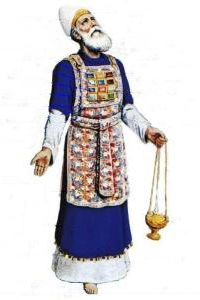
\includegraphics[width=50mm,scale=1.5]{Extras/Melchisedec.jpg}
\vspace{0.4in}  % Create a title for the document and write it in bold font
\LARGE{\textbf{\date}} % Again, do a line break
\linebreak 
% Create a subtitle \large{with Outlines, Statistics, Cross References, and Notes}
\vspace{0.5in}
\begin{flushleft}
\LARGE{Day \#82: Wednesday, 23  March 2022 PLAIN  \\}\vspace{0.25in}
\LARGE{1 Samuel 1-3 Psalm 82 Proverb 23}
\end{flushleft}
\vspace{0.6in}
\bigskip

\normalsize{Xenia, Oh.\\}
\normalsize{created: \today}
\vspace{1.3in}

\end{flushright}
\end{titlepage}

\newpage 
\tableofcontents\hypertarget{TOC}{}
\listoffigures
\listoftables

\hyphenation{A-bim-e-lech bre-thren E-phra-im  Gib-e-o-nites Jer-u-sa-lem through-out Phil-i-stines The-o-phil-us Am-a-le-kites ven-geance Mesh-el-e-mi-ah onan-ism Phar-a-oh thoughts grev-ous-ness Hach-a-liah adul-ter-er Shad-rach}

%%%%%%%%%%%%%%%%% EXTRA COLORS
%%%%%%%%%%%%%%%%% EXTRA COLORS
%%%%%%%%%%%%%%%%% EXTRA COLORS
\definecolor{champagne}{rgb}{0.97,0.91,0.81}
\definecolor{bone}{rgb}{0.89,0.85,0.79}

\definecolor{ForestGreen}{rgb}{0.00,0.29,0.098}
\definecolor{GIVING}{cmyk}{1,0.0,0.72,.1}

\definecolor{MLPE}{cmyk}{1,1,0,.45}
\definecolor{SOCCER}{cmyk}{.77, 0, .42, .49}
\definecolor{PAYBILL}{cmyk}{0,0.83,0.76,0.07}
\definecolor{SERMON}{cmyk}{.14,.9,0,.30} % aka seance \href{http://www.flatuicolorpicker.com/purple-cmyk-color-model/}{seance}
\definecolor{BIBLE}{cmyk}{0,.17,.74,.17}
\definecolor{WORKBLUE}{cmyk}{1, .5, 0, .6}
\definecolor{myOrange}{cmyk}{0, .4, .98, .03}
\definecolor{myTan}{cmyk}{0.0,.07,.17,.10}
\definecolor{myRed}{cmyk}{0,1,1,0}
\definecolor{myWhite}{cmyk}{0,0,0,0}
\definecolor{BLUESoD}{cmyk}{.97,.84,0,.04}
\definecolor{WHITE}{cmyk}{0,0,0,0}
\definecolor{OLDGOLD}{cmyk}{0.05,0.3,1.00,0}
\definecolor{CASTLETON}{cmyk}{1,0,0.31,0.66}
\definecolor{cadmiumgreen}{rgb}{0.0, 0.42, 0.24}
\definecolor{jungle}{rgb}{0.203,0.4882,0.1718}
\definecolor{MYGOLD}{rgb}{1,.84,0}

\definecolor{MYLIGHTGRAY}{rgb}{.85,.85,.85}

\definecolor{codegreen}{rgb}{0,0.6,0}
\definecolor{codegray}{rgb}{0.5,0.5,0.5}
\definecolor{codepurple}{rgb}{0.58,0,0.82}
\definecolor{backcolour}{rgb}{0.95,0.95,0.92}


\mdfdefinestyle{MyFrame}{%
    linecolor=blue,
    outerlinewidth=2pt,
    roundcorner=5pt,
    innertopmargin=\baselineskip,
    innerbottommargin=\baselineskip,
    innerrightmargin=10pt,
    innerleftmargin=10pt,
    backgroundcolor=gray!25!white}


\mdfdefinestyle{MyFrame2}{%
    linecolor=black,
    outerlinewidth=2pt,
    roundcorner=5pt,
    innertopmargin=\baselineskip,
    innerbottommargin=\baselineskip,
    innerrightmargin=10pt,
    innerleftmargin=10pt,
    backgroundcolor=yellow!25!white}


%%%%%
%% for PFTTIS list
%%%%%

%%% And Joseph said unto
\index[PFTTIS]{And Joseph said unto!Genesis!Gen 40:008}
\index[PFTTIS]{And Joseph said unto!Genesis!Gen 40:012}
\index[PFTTIS]{And Joseph said unto!Genesis!Gen 41:025}
\index[PFTTIS]{And Joseph said unto!Genesis!Gen 42:014}
\index[PFTTIS]{And Joseph said unto!Genesis!Gen 42:018}
\index[PFTTIS]{And Joseph said unto!Genesis!Gen 44:015}
\index[PFTTIS]{And Joseph said unto!Genesis!Gen 45:003}
\index[PFTTIS]{And Joseph said unto!Genesis!Gen 45:004}
\index[PFTTIS]{And Joseph said unto!Genesis!Gen 46:031}
\index[PFTTIS]{And Joseph said unto!Genesis!Gen 48:009}
\index[PFTTIS]{And Joseph said unto!Genesis!Gen 48:018}
\index[PFTTIS]{And Joseph said unto!Genesis!Gen 50:019}
\index[PFTTIS]{And Joseph said unto!Genesis!Gen 50:024}


%%% a shadow
\index[PFTTIS]{a shadow!1Chronicles!1Chr 029:15}
\index[PFTTIS]{a shadow!Job!Job 008:09}
\index[PFTTIS]{a shadow!Job!Job 014:02}
\index[PFTTIS]{a shadow!Job!Job 017:07}
\index[PFTTIS]{a shadow!Psalm!Psa 102:011}
\index[PFTTIS]{a shadow!Psalm!Psa 144:004}
\index[PFTTIS]{a shadow!Ecclesiastes!Eccl 006:012}
\index[PFTTIS]{a shadow!Ecclesiastes!Eccl 008:013}
\index[PFTTIS]{a shadow!Isaiah!Isa 04:006}
\index[PFTTIS]{a shadow!Isaiah!Isa 25:004}
\index[PFTTIS]{a shadow!Jonah!Jnh 04:06}
\index[PFTTIS]{a shadow!Colossians!Col 02:017}
\index[PFTTIS]{a shadow!Hebews!Heb 10:001}

%%% blessed is the man
\index[PFTTIS]{blessed is the man!Psalm!Psa 001:001}
\index[PFTTIS]{blessed is the man!Psalm!Psa 032:002}
\index[PFTTIS]{blessed is the man!Psalm!Psa 034:008}
\index[PFTTIS]{blessed is the man!Psalm!Psa 065:004}
\index[PFTTIS]{blessed is the man!Psalm!Psa 084:005}
\index[PFTTIS]{blessed is the man!Psalm!Psa 084:012}
\index[PFTTIS]{blessed is the man!Psalm!Psa 094:012}
\index[PFTTIS]{blessed is the man!Psalm!Psa 112:001}
\index[PFTTIS]{blessed is the man!Proverbs!Pro 008:034}
\index[PFTTIS]{blessed is the man!Isaiah!Isa 056:002}
\index[PFTTIS]{blessed is the man!Jeremiah!Jer 017:007}
\index[PFTTIS]{blessed is the man!Romans!Rom 004:008}
\index[PFTTIS]{blessed is the man!James!Jam 001:012}


%%% carry them
\index[PFTTIS]{carry them!Leviticus!Lev 14:045}
\index[PFTTIS]{carry them!Numbers!Num 11:012}
\index[PFTTIS]{carry them!Joshua!Jsh 04:003}
\index[PFTTIS]{carry them!1Samuel!1Sam 20:040}
\index[PFTTIS]{carry them!1Kings!1Kng 08:046}
\index[PFTTIS]{carry them!2Chronicles!2Chr 06:036}
\index[PFTTIS]{carry them!Ezra!Ezra 05:015}
\index[PFTTIS]{carry them!Isaiah!Isa 40:011}
\index[PFTTIS]{carry them!Isaiah!Isa 41:016}
\index[PFTTIS]{carry them!Isaiah!Isa 57:013}
\index[PFTTIS]{carry them!Jeremiah!Jer 20:004}
\index[PFTTIS]{carry them!Jeremiah!Jer 20:005}
\index[PFTTIS]{carry them!Jeremiah!Jer 43:012}


\index[PFTTIS]{good tidings!2Samuel!2Sam 18:027}
\index[PFTTIS]{good tidings!1Kings!1Ki 01:042}
\index[PFTTIS]{good tidings!2Kings!2Ki 07:009 (2x)}
\index[PFTTIS]{good tidings!Isaiah!Isa 40:009 (2x)}
\index[PFTTIS]{good tidings!Isaiah!Isa 41:007}
\index[PFTTIS]{good tidings!Isaiah!Isa 52:007}
\index[PFTTIS]{good tidings!Isaiah!Isa 61:001}
\index[PFTTIS]{good tidings!Nahum!Nah 01:005}
\index[PFTTIS]{good tidings!Luke!Lk 02:010}
\index[PFTTIS]{good tidings!1Thessalonians!1Thess 03:006}


%%% dead body
\index[PFTTIS]{dead body!Leviticus!Lev 21:011}
\index[PFTTIS]{dead body!Numbers!Num 06:006}
\index[PFTTIS]{dead body!Numbers!Num 09:006}
\index[PFTTIS]{dead body!Numbers!Num 09:007}
\index[PFTTIS]{dead body!Numbers!Num 09:010}
\index[PFTTIS]{dead body!Numbers!Num 09:011}
\index[PFTTIS]{dead body!Numbers!Num 09:013}
\index[PFTTIS]{dead body!Numbers!Num 09:016}
\index[PFTTIS]{dead body!2Kings!2Ki 08:005}
\index[PFTTIS]{dead body!Isaiah!Isa 26:019}
\index[PFTTIS]{dead body!Jeremiah!Jer 26:023}
\index[PFTTIS]{dead body!Jeremiah!Jer 36:030}
\index[PFTTIS]{dead body!Haggai!Hag 02:013}

%%% great sea
\index[PFTTIS]{great sea!Numbers!Num 34:006}
\index[PFTTIS]{great sea!Numbers!Num 34:007}
\index[PFTTIS]{great sea!Joshua!Jos 01:004}
\index[PFTTIS]{great sea!Joshua!Jos 09:001}
\index[PFTTIS]{great sea!Joshua!Jos 15:012}
\index[PFTTIS]{great sea!Joshua!Jos 15:047}
\index[PFTTIS]{great sea!Joshua!Jos 23:004}
\index[PFTTIS]{great sea!Ezekiel!Eze 47:010}
\index[PFTTIS]{great sea!Ezekiel!Eze 47:015}
\index[PFTTIS]{great sea!Ezekiel!Eze 47:019}
\index[PFTTIS]{great sea!Ezekiel!Eze 47:020}
\index[PFTTIS]{great sea!Ezekiel!Eze 48:028}
\index[PFTTIS]{great sea!Daniel!Dan 07:002}


%%% have forsaken me
\index[PFTTIS]{have forsaken me!Judges!Jdg 10:013}
\index[PFTTIS]{have forsaken me!1Samuel!1Sam 08:008}
\index[PFTTIS]{have forsaken me!1Kings!1Ki 11:033}
\index[PFTTIS]{have forsaken me!2Kings!2Ki 22:017}
\index[PFTTIS]{have forsaken me!2Chronicles!2Chr 12:005}
\index[PFTTIS]{have forsaken me!2Chronicles!2Chr 34:025}
\index[PFTTIS]{have forsaken me!Jeremiah!Jer 01:016}
\index[PFTTIS]{have forsaken me!Jeremiah!Jer 02:013}
\index[PFTTIS]{have forsaken me!Jeremiah!Jer 05:007}
\index[PFTTIS]{have forsaken me!Jeremiah!Jer 05:019}
\index[PFTTIS]{have forsaken me!Jeremiah!Jer 16:011 (2x)}
\index[PFTTIS]{have forsaken me!Jeremiah!Jer 19:004}

%%% no king
\index[PFTTIS]{no king!Judges!Jdg 17:06}
\index[PFTTIS]{no king!Judges!Jdg 18:01}
\index[PFTTIS]{no king!Judges!Jdg 19:01}
\index[PFTTIS]{no king!Judges!Jdg 21:25}
\index[PFTTIS]{no king!1Kings!1Ki 22:47}
\index[PFTTIS]{no king!2Kings!2Ki 23:25}
\index[PFTTIS]{no king!Nehemiah!Neh 13:26}
\index[PFTTIS]{no king!Psalms!Psa 033:016}
\index[PFTTIS]{no king!Proverbs!Pro 30:27}
\index[PFTTIS]{no king!Daniel!Dan 02:10}
\index[PFTTIS]{no king!Hosea!Hos 10:03}
\index[PFTTIS]{no king!Micah!Mic 04:09}
\index[PFTTIS]{no king!John!Jhn 19:15}


%%% rebellious house
\index[PFTTIS]{rebellious house!Exodus!Exo 02:005}
\index[PFTTIS]{rebellious house!Exodus!Exo 02:006}
\index[PFTTIS]{rebellious house!Exodus!Exo 02:008}
\index[PFTTIS]{rebellious house!Exodus!Exo 03:009}
\index[PFTTIS]{rebellious house!Exodus!Exo 03:026}
\index[PFTTIS]{rebellious house!Exodus!Exo 03:027}
\index[PFTTIS]{rebellious house!Exodus!Exo 12:002 (2x)}
\index[PFTTIS]{rebellious house!Exodus!Exo 12:003}
\index[PFTTIS]{rebellious house!Exodus!Exo 12:009}
\index[PFTTIS]{rebellious house!Exodus!Exo 12:025}
\index[PFTTIS]{rebellious house!Exodus!Exo 17:012}
\index[PFTTIS]{rebellious house!Exodus!Exo 24:003}

%%% seek him
\index[PFTTIS]{seek him!Deuteronomy!Deu 04:029}\index[PFTTIS]{seek him!1Samuel!1Sam 23:025}
\index[PFTTIS]{seek him!1Chronicles!1Chr 28:009}
\index[PFTTIS]{seek him!2Chronicles!1Chr 15:002}
\index[PFTTIS]{seek him!Ezra!Ezr 08:022}
\index[PFTTIS]{seek him!Psalms!Psa 022:026}
\index[PFTTIS]{seek him!Psalms!Psa 024:006}
\index[PFTTIS]{seek him!Psalms!Psa 119:002}
\index[PFTTIS]{seek him!SoS!SoS 03:002}
\index[PFTTIS]{seek him!SoS!SoS 06:001}
\index[PFTTIS]{seek him!Hosea!Hos 07:010}
\index[PFTTIS]{seek him!Amos!Amo 05:008}
\index[PFTTIS]{seek him!Hebrews!Heb 11:0063}


%%% seek ye
\index[PFTTIS]{seek ye!Isaiah!Isa 34:016}
\index[PFTTIS]{seek ye!Isaiah!Isa 45:019}
\index[PFTTIS]{seek ye!Isaiah!Isa 55:006}
\index[PFTTIS]{seek ye!Amos!Amos 5:004}
\index[PFTTIS]{seek ye!John!John 1:38}
\index[PFTTIS]{seek ye!John!John 18:4}
\index[PFTTIS]{seek ye!John!John 18:7}
\index[PFTTIS]{seek ye!Matthew!Matt 6:33}
\index[PFTTIS]{seek ye!Numbers!Num 16:10}
\index[PFTTIS]{seek ye!Luke!Luke 12:31}
\index[PFTTIS]{seek ye!Luke!Luke 24:5}
\index[PFTTIS]{seek ye!Psalm!Psa 27:8}
\index[PFTTIS]{seek ye!Zephaniah!Zeph 2:3}

%%% the uncircumcised
\index[PFTTIS]{the uncircumcised!Genesis!Gen 17:014}
\index[PFTTIS]{the uncircumcised!Judges!Jdg 14:003}
\index[PFTTIS]{the uncircumcised!Judges!Jdg 15:018}
\index[PFTTIS]{the uncircumcised!2Samuel!2Sam 01:020}
\index[PFTTIS]{the uncircumcised!Isaiah!Isa 02:001}
\index[PFTTIS]{the uncircumcised!Jeremiah!Jer 09:025}
\index[PFTTIS]{the uncircumcised!Ezekiel!Eze 28:010}
\index[PFTTIS]{the uncircumcised!Ezekiel!Eze 31:018}
\index[PFTTIS]{the uncircumcised!Ezekiel!Eze 32:019}
\index[PFTTIS]{the uncircumcised!Ezekiel!Eze 32:027}
\index[PFTTIS]{the uncircumcised!Ezekiel!Eze 32:028}
\index[PFTTIS]{the uncircumcised!Ezekiel!Eze 32:029}
\index[PFTTIS]{the uncircumcised!Ezekiel!Eze 32:032}

%%% worship him
\index[PFTTIS]{worship him!Psalms!Psa 97:007}
\index[PFTTIS]{worship him!Zephaniah!Zeph 02:011}
\index[PFTTIS]{worship him!Matthew!Matt 02:002}
\index[PFTTIS]{worship him!Matthew!Matt 02:008}
\index[PFTTIS]{worship him!John!John 04:023}
\index[PFTTIS]{worship him!John!John 04:024 (2x)} 
\index[PFTTIS]{worship him!Acts!Acts 17:023}
\index[PFTTIS]{worship him!Hebrews!Heb 01:006}
\index[PFTTIS]{worship him!Revelation!Rev 04:010}
\index[PFTTIS]{worship him!Revelation!Rev 13:008}
\index[PFTTIS]{worship him!Revelation!Rev 14:007}
\index[PFTTIS]{worship him!Revelation!Rev 19:010}


%%%%%
%% for PFTTIS list
%%%%%

%%% afflictions
\index[WFTTIS]{afflictions!Psalms!Psa 34:019}
\index[WFTTIS]{afflictions!Psalms!Psa 132:001}
\index[WFTTIS]{afflictions!Acts!Acts 07:010}
\index[WFTTIS]{afflictions!Acts!Acts 20:023}
\index[WFTTIS]{afflictions!2Corinthians!2Cor 06:004}
\index[WFTTIS]{afflictions!Colossians!Col 01:024}
\index[WFTTIS]{afflictions!1Thessalonians!1Thess 03:003}
\index[WFTTIS]{afflictions!2Timothy!2Tim 01:008}
\index[WFTTIS]{afflictions!2Timothy!2Tim 03:011}
\index[WFTTIS]{afflictions!2Timothy!2Tim 04:005}
\index[WFTTIS]{afflictions!Hebrews!Heb 10:032}
\index[WFTTIS]{afflictions!Hebrews!Heb 10:033}
\index[WFTTIS]{afflictions!1Peter!1Pet 05:009}

%%% acsend
\index[WFTTIS]{acsend!Joshua!Jos 06:05}
\index[WFTTIS]{acsend!Psalm!Psa 024:003}
\index[WFTTIS]{acsend!Psalm!Psa 135:007}
\index[WFTTIS]{acsend!Psalm!Psa 139:008}
\index[WFTTIS]{acsend!Isaiah!Isa 14:013}
\index[WFTTIS]{acsend!Isaiah!Isa 14:014}
\index[WFTTIS]{acsend!Jeremiah!Jer 10:013}
\index[WFTTIS]{acsend!Jeremiah!Jer 51:016}
\index[WFTTIS]{acsend!Ezekiel!Eze 38:009}
\index[WFTTIS]{acsend!John!John 06:062}
\index[WFTTIS]{acsend!John!John 20:017}
\index[WFTTIS]{acsend!Romans!Rom 10:006}
\index[WFTTIS]{acsend!Revelation!Rev 17:008}

%%% Assyrian
\index[WFTTIS]{Assyrian!Isaiah!Isa 10:005}
\index[WFTTIS]{Assyrian!Isaiah!Isa 10:024}
\index[WFTTIS]{Assyrian!Isaiah!Isa 14:025}
\index[WFTTIS]{Assyrian!Isaiah!Isa 19:023}
\index[WFTTIS]{Assyrian!Isaiah!Isa 23:013}
\index[WFTTIS]{Assyrian!Isaiah!Isa 30:031}
\index[WFTTIS]{Assyrian!Isaiah!Isa 31:008}
\index[WFTTIS]{Assyrian!Isaiah!Isa 52:004}
\index[WFTTIS]{Assyrian!Ezekiel!Eze 31:003}
\index[WFTTIS]{Assyrian!Hosea!Hos 05:013}
\index[WFTTIS]{Assyrian!Hosea!Hos 11:005}
\index[WFTTIS]{Assyrian!Micah!Hos 05:005}
\index[WFTTIS]{Assyrian!Micah!Hos 05:006}

%%% blot
\index[WFTTIS]{blot!Exodus!Exo 32:032}
\index[WFTTIS]{blot!Exodus!Exo 32:033}
\index[WFTTIS]{blot!Numbers!Num 05:026}
\index[WFTTIS]{blot!Deuteronomy!Deut 09:014}
\index[WFTTIS]{blot!Deuteronomy!Deut 25:019}
\index[WFTTIS]{blot!Deuteronomy!Deut 29:020}
\index[WFTTIS]{blot!2Kings!2Ki 14:027}
\index[WFTTIS]{blot!Job!Job 31:007}
\index[WFTTIS]{blot!Psalms!Psa 51:001}
\index[WFTTIS]{blot!Psalms!Psa 51:009}
\index[WFTTIS]{blot!Proverbs!Pro 09:007}
\index[WFTTIS]{blot!Jeremiah!Jer 18:023}
\index[WFTTIS]{blot!Revelation!Rev 03:005}


%%% chain
\index[WFTTIS]{chain!Genesis!Gen 41:042}
\index[WFTTIS]{chain!1Kings!1Ki 07:017}
\index[WFTTIS]{chain!Psalms!Psa 73:006}
\index[WFTTIS]{chain!SoS!Sos 04:009}
\index[WFTTIS]{chain!Lamentations!Lam 03:007}
\index[WFTTIS]{chain!Ezekiel!Eze 07:023}
\index[WFTTIS]{chain!Ezekiel!Eze 16:011}
\index[WFTTIS]{chain!Daniel!Dan 05:007}
\index[WFTTIS]{chain!Daniel!Dan 05:016}
\index[WFTTIS]{chain!Daniel!Dan 05:029}
\index[WFTTIS]{chain!Acts!Acts 28:020}
\index[WFTTIS]{chain!2Timothy!2Tim 01:016}
\index[WFTTIS]{chain!Revelation!Rev 20:001}


%%% controversy
\index[WFTTIS]{controversy!Deuteronomy!Deu 17:008}
\index[WFTTIS]{controversy!Deuteronomy!Deu 19:017}
\index[WFTTIS]{controversy!Deuteronomy!Deu 21:005}
\index[WFTTIS]{controversy!Deuteronomy!Deu 25:001}
\index[WFTTIS]{controversy!2Samuel!2Sam 15:002}
\index[WFTTIS]{controversy!Isaiah!Isa 34:008}
\index[WFTTIS]{controversy!Jeremiah!Jer 25:031}
\index[WFTTIS]{controversy!Ezekiel!Eze 44:024}
\index[WFTTIS]{controversy!Hosea!Hos 04:001}
\index[WFTTIS]{controversy!Hosea!Hos 12:002}
\index[WFTTIS]{controversy!Micah!Mic 06:002 (2x)}
\index[WFTTIS]{controversy!1Timothy!1Tim 03:016}


%%% Dagon/Dagon's
\index[WFTTIS]{Dagon!Judges!Jdg 16:023}
\index[WFTTIS]{Dagon!1Samuel!1Sam 05:002 (2x)}
\index[WFTTIS]{Dagon!1Samuel!1Sam 05:003 (2x)}
\index[WFTTIS]{Dagon!1Samuel!1Sam 05:004 (3x)}
\index[WFTTIS]{Dagon!1Samuel!1Sam 05:005 (3x)}
\index[WFTTIS]{Dagon!1Samuel!1Sam 05:007}
\index[WFTTIS]{Dagon!1Chronicles!1Chr 10:010}

%%% disobedient
\index[WFTTIS]{disobedient!1Kings!1Ki 13:026}
\index[WFTTIS]{disobedient!Nehemiah!Neh 09:026}
\index[WFTTIS]{disobedient!Luke!Luke 01:017}
\index[WFTTIS]{disobedient!Acts!Acts 26:019}
\index[WFTTIS]{disobedient!Romans!Rom 01:030}
\index[WFTTIS]{disobedient!Romans!Rom 10:021}
\index[WFTTIS]{disobedient!1Timothy!1Tim 01:009}
\index[WFTTIS]{disobedient!2Timothy!2Tim 03:002}
\index[WFTTIS]{disobedient!Titus!Titus 01:016}
\index[WFTTIS]{disobedient!Titus!Titus 03:003}
\index[WFTTIS]{disobedient!1Peter!1Pet 02:007}
\index[WFTTIS]{disobedient!1Peter!1Pet 02:008}
\index[WFTTIS]{disobedient!1Peter!1Pet 03:020}


%%% doubt
\index[WFTTIS]{doubt!Genesis!Gen 37:033}
\index[WFTTIS]{doubt!Deuteronomy!Deu 28:066}
\index[WFTTIS]{doubt!Job!Job 12:002}
\index[WFTTIS]{doubt!Matthew!Matt 14:031}
\index[WFTTIS]{doubt!Matthew!Matt 21:021}
\index[WFTTIS]{doubt!Mark!Mk 11:023}
\index[WFTTIS]{doubt!Luke!Lk 11:020}
\index[WFTTIS]{doubt!John!Jhn 10:024}
\index[WFTTIS]{doubt!Acts!Acts 02:012}
\index[WFTTIS]{doubt!Acts!Acts 28:004}
\index[WFTTIS]{doubt!1Corinthians!1Cor 09:010}
\index[WFTTIS]{doubt!Galatians!Gal 04:020}
\index[WFTTIS]{doubt!1John!1Jhn 02:019}


%%% dungeon
\index[WFTTIS]{dungeon!Genesis!Gen 40:015}
\index[WFTTIS]{dungeon!Genesis!Gen 41:014}
\index[WFTTIS]{dungeon!Exodus!Exo 12:029}
\index[WFTTIS]{dungeon!Jeremiah!Jer 37:016}
\index[WFTTIS]{dungeon!Jeremiah!Jer 38:006 (2x)}
\index[WFTTIS]{dungeon!Jeremiah!Jer 38:007}
\index[WFTTIS]{dungeon!Jeremiah!Jer 38:009}
\index[WFTTIS]{dungeon!Jeremiah!Jer 38:010}
\index[WFTTIS]{dungeon!Jeremiah!Jer 38:011}
\index[WFTTIS]{dungeon!Jeremiah!Jer 38:013}
\index[WFTTIS]{dungeon!Lamentations!Lam 03:053}
\index[WFTTIS]{dungeon!Lamentations!Lam 03:055}


%%% error
\index[WFTTIS]{error!2Samuel!2Sam 06:007}
\index[WFTTIS]{error!Job!Job 19:004}
\index[WFTTIS]{error!Ecclesiastes!Ecc 05:006}
\index[WFTTIS]{error!Ecclesiastes!Ecc 10:005}
\index[WFTTIS]{error!Isaiah!Isa 32:006}
\index[WFTTIS]{error!Daniel!Dan 06:004}
\index[WFTTIS]{error!Matthew!Matt 27:064}
\index[WFTTIS]{error!Romans!Rom 01:027}
\index[WFTTIS]{error!James!Jam 05:020}
\index[WFTTIS]{error!2Peter!2Pet 02:018}
\index[WFTTIS]{error!2Peter!2Pet 03:017}
\index[WFTTIS]{error!1John!1Jn 04:006}
\index[WFTTIS]{error!Jude!Jude 01:011}

%%% fourish
\index[WFTTIS]{fourish!Psalms!Psa 072:007}
\index[WFTTIS]{fourish!Psalms!Psa 072:016}
\index[WFTTIS]{fourish!Psalms!Psa 092:007}
\index[WFTTIS]{fourish!Psalms!Psa 092:012}
\index[WFTTIS]{fourish!Psalms!Psa 092:013}
\index[WFTTIS]{fourish!Psalms!Psa 132:018}
\index[WFTTIS]{fourish!Proverbs!Pro 11:28}
\index[WFTTIS]{fourish!Proverbs!Pro 14:11}
\index[WFTTIS]{fourish!Ecclesiastes!Ecc 12:05}
\index[WFTTIS]{fourish!SongOfSolomon!SOS 07:12}
\index[WFTTIS]{fourish!Isaiah!Isa 17:11}
\index[WFTTIS]{fourish!Isaiah!Isa 66:14}
\index[WFTTIS]{fourish!Ezekiel!Eze 17:24}




%%% giants
\index[WFTTIS]{giants!Genesis!Gen 06:004}
\index[WFTTIS]{giants!Numbers!Num 13:033}
\index[WFTTIS]{giants!Deuteronomy!Deut 02:011}
\index[WFTTIS]{giants!Deuteronomy!Deut 02:021}
\index[WFTTIS]{giants!Deuteronomy!Deut 03:011}
\index[WFTTIS]{giants!Deuteronomy!Deut 03:013}
\index[WFTTIS]{giants!Joshua!Josh 12:004}
\index[WFTTIS]{giants!Joshua!Josh 13:012}
\index[WFTTIS]{giants!Joshua!Josh 15:008}
\index[WFTTIS]{giants!Joshua!Josh 17:015}
\index[WFTTIS]{giants!Joshua!Josh 16:016}

%%% good man
\index[WFTTIS]{good man!2 Samuel!2Sa 18:27}
%(1) Psalms 37:23 [5]
%(1) Psalms 112:5 [2]
%(1) Proverbs 12:2 [2]
%(1) Proverbs 13:22 [2]
%(1) Proverbs 14:14 [14]
%(1) Micah 7:2 [2]
%(1) Matthew 12:35 [2]
%(1) Luke 6:45 [2]
%(1) Luke 23:50 [15]
%(1) John 7:12 [17]
%(1) Acts 11:24 [5]
%(1) Romans 5:7 [14]

%%% Hinnom
\index[WFTTIS]{Hinnom!Joshua!Jsh 15:008}
\index[WFTTIS]{Hinnom!Joshua!Jsh 18:016}
\index[WFTTIS]{Hinnom!2Kings!2Ki 23:010}
\index[WFTTIS]{Hinnom!2Chronicles!2Chr 28:003}
\index[WFTTIS]{Hinnom!2Chronicles!2Chr 33:006}
\index[WFTTIS]{Hinnom!Nehemiah!Neh 11:030}
\index[WFTTIS]{Hinnom!Jeremiah!Jer 07:031}
\index[WFTTIS]{Hinnom!Jeremiah!Jer 07:032}
\index[WFTTIS]{Hinnom!Jeremiah!Jer 19:002}
\index[WFTTIS]{Hinnom!Jeremiah!Jer 19:006}
\index[WFTTIS]{Hinnom!Jeremiah!Jer 32:035}

%%% inclined
\index[WFTTIS]{inclined!Judges!Jdg 09:003}
\index[WFTTIS]{inclined!Psalms!Psa 040:001}
\index[WFTTIS]{inclined!Psalms!Psa 116:002}
\index[WFTTIS]{inclined!Psalms!Psa 119:112}
\index[WFTTIS]{inclined!Proverbs!Pro 05:13}
\index[WFTTIS]{inclined!Jeremiah!Jer 07:24}
\index[WFTTIS]{inclined!Jeremiah!Jer 07:26}
\index[WFTTIS]{inclined!Jeremiah!Jer 11:08}
\index[WFTTIS]{inclined!Jeremiah!Jer 17:23}
\index[WFTTIS]{inclined!Jeremiah!Jer 25:04}
\index[WFTTIS]{inclined!Jeremiah!Jer 34:14}
\index[WFTTIS]{inclined!Jeremiah!Jer 35:15}
\index[WFTTIS]{inclined!Jeremiah!Jer 44:05}


%%% laughed
\index[WFTTIS]{laughed!Genesis!Gen 17:017}
\index[WFTTIS]{laughed!Genesis!Gen 18:012}
\index[WFTTIS]{laughed!Genesis!Gen 18:015}
\index[WFTTIS]{laughed!2Kings!2Ki 19:021}
\index[WFTTIS]{laughed!2Chronicles!2Chr 30:010}
\index[WFTTIS]{laughed!Nehemiah!Neh 02:019}
\index[WFTTIS]{laughed!Job!Job 12:004}
\index[WFTTIS]{laughed!Job!Job 29:024}
\index[WFTTIS]{laughed!Isaiah!Isa 37:022}
\index[WFTTIS]{laughed!Ezekiel!Ezek 23:032}
\index[WFTTIS]{laughed!Matthew!Matt 09:024}
\index[WFTTIS]{laughed!Mark!Mk 05:040}
\index[WFTTIS]{laughed!Luke!Lk 08:053}

%%% liar
\index[WFTTIS]{liar!Job!Job 24:025}
\index[WFTTIS]{liar!Proverbs!Pro 17:004}
\index[WFTTIS]{liar!Proverbs!Pro 19:022}
\index[WFTTIS]{liar!Proverbs!Pro 30:006}
\index[WFTTIS]{liar!Jeremiah!Jer 15:018}
\index[WFTTIS]{liar!John!Jhn 08:044}
\index[WFTTIS]{liar!John!Jhn 08:055}
\index[WFTTIS]{liar!Romans!Rom 03:004}
\index[WFTTIS]{liar!1John!1Jhn 01:010}
\index[WFTTIS]{liar!1John!1Jhn 02:004}
\index[WFTTIS]{liar!1John!1Jhn 02:022}
\index[WFTTIS]{liar!1John!1Jhn 04:020}
\index[WFTTIS]{liar!1John!1Jhn 05:010}

%%% palsy
\index[WFTTIS]{palsy!Matthew!Matt 04:024}
\index[WFTTIS]{palsy!Matthew!Matt 08:006}
\index[WFTTIS]{palsy!Matthew!Matt 09:002}
\index[WFTTIS]{palsy!Matthew!Matt 09:006}
\index[WFTTIS]{palsy!Mark!Mk 02:003}
\index[WFTTIS]{palsy!Mark!Mk 02:004}
\index[WFTTIS]{palsy!Mark!Mk 02:005}
\index[WFTTIS]{palsy!Mark!Mk 02:009}
\index[WFTTIS]{palsy!Mark!Mk 02:010}
\index[WFTTIS]{palsy!Luke!Lk 05:018}
\index[WFTTIS]{palsy!Luke!Lk 05:024}
\index[WFTTIS]{palsy!Acts!Acts 09:033}

%%% Profitable
\index[WFTTIS]{profitable!Job!Job 22:002 (2x)}
\index[WFTTIS]{profitable!Ecclesiastes!Ecc 10:010}
\index[WFTTIS]{profitable!Isaiah!Isa 44:010}
\index[WFTTIS]{profitable!Jeremiah!Jer 13:007}
\index[WFTTIS]{profitable!Matthew!Matt 05:029}
\index[WFTTIS]{profitable!Matthew!Matt 05:030}
\index[WFTTIS]{profitable!Acts!Acts 20:020}
\index[WFTTIS]{profitable!1Timothy!1Tim 04:008}
\index[WFTTIS]{profitable!2Timothy!2Tim 03:016}
\index[WFTTIS]{profitable!2Timothy!2Tim 04:011}
\index[WFTTIS]{profitable!Titus!Titus 03:008}
\index[WFTTIS]{profitable!Philemon!Phlm 01:011}

%%% Rechab
\index[WFTTIS]{Rechab!2Samuel!2Sam 04:002}
\index[WFTTIS]{Rechab!2Samuel!2Sam 04:005}
\index[WFTTIS]{Rechab!2Samuel!2Sam 04:006}
\index[WFTTIS]{Rechab!2Samuel!2Sam 04:009}
\index[WFTTIS]{Rechab!2KIngs!2Ki 10:015}
\index[WFTTIS]{Rechab!2KIngs!2Ki 10:023}
\index[WFTTIS]{Rechab!1Chronicles!1Chr 02:055}
\index[WFTTIS]{Rechab!Nehemiah!Neh 03:014}
\index[WFTTIS]{Rechab!Jeremiah!Jer 35:006}
\index[WFTTIS]{Rechab!Jeremiah!Jer 35:008}
\index[WFTTIS]{Rechab!Jeremiah!Jer 35:014}
\index[WFTTIS]{Rechab!Jeremiah!Jer 35:016}
\index[WFTTIS]{Rechab!Jeremiah!Jer 35:019}

%%% serpents
\index[WFTTIS]{serpents!Exodus!Exo 07:012}
\index[WFTTIS]{serpents!Numbers!Num 21:006}
\index[WFTTIS]{serpents!Numbers!Num 21:007}
\index[WFTTIS]{serpents!Deuteronomy!Deu 08:015}
\index[WFTTIS]{serpents!Deuteronomy!Deu 32:024}
\index[WFTTIS]{serpents!Jeremiah!Jer 08:017}
\index[WFTTIS]{serpents!Matthew!Matt 10:016}
\index[WFTTIS]{serpents!Matthew!Matt 23:033}
\index[WFTTIS]{serpents!Mark!Mk 16:018}
\index[WFTTIS]{serpents!Luke!Lk 10:019}
\index[WFTTIS]{serpents!1Corinthians!1Cor 10:009}
\index[WFTTIS]{serpents!James!Jas 03:007}
\index[WFTTIS]{serpents!Revelation!Rev 09:019}

%%% short
\index[WFTTIS]{short!Numbers!Num 11:023}
\index[WFTTIS]{short!2Kings!2Ki 10:032}
\index[WFTTIS]{short!Job!Job 17:012}
\index[WFTTIS]{short!Job!Job 20:005}
\index[WFTTIS]{short!Psalms!Psa 89:047}
\index[WFTTIS]{short!Romans!Rom 03:023}
\index[WFTTIS]{short!Romans!Rom 09:028  (2x)}
\index[WFTTIS]{short!1Corinthians!1Cor 07:029}
\index[WFTTIS]{short!1Thessalonians!1Thess 02:017}
\index[WFTTIS]{short!Hebrews!Heb 04:001}
\index[WFTTIS]{short!Revelation!Rev 12:012}
\index[WFTTIS]{short!Revelation!Rev 17:010}

%%% smiteth
\index[WFTTIS]{smiteth!Exodus!Exo 21:012}
\index[WFTTIS]{smiteth!Exodus!Exo 21:15}
\index[WFTTIS]{smiteth!Deuteronomy!Dt 25:11}
\index[WFTTIS]{smiteth!Deuteronomy!Dt 27:24}
\index[WFTTIS]{smiteth!Joshua!Jsh 15:16}
\index[WFTTIS]{smiteth!Judges!Jdg 15:16}
\index[WFTTIS]{smiteth!2 Samuel!2Sa 05:08}
\index[WFTTIS]{smiteth!1Chronicles!1Chr 11:06}
\index[WFTTIS]{smiteth!Job!1Chr 26:12}
\index[WFTTIS]{smiteth!Isaiah!Isa 09:13}
\index[WFTTIS]{smiteth!Lamentations!Lam 03:30}
\index[WFTTIS]{smiteth!Ezekiel!Eze 07:09}
\index[WFTTIS]{smiteth!Luke!Lk 06:29}



%%% vanities
\index[WFTTIS]{vanities!Deuteronomy!Deut 21:021}
\index[WFTTIS]{vanities!1Kings!1Ki 16:013}
\index[WFTTIS]{vanities!1Kings!1Ki 16:026}
\index[WFTTIS]{vanities!Psalms!Psa 031:006}
\index[WFTTIS]{vanities!Ecclesiastes!Ecc 01:002 (2x)}
\index[WFTTIS]{vanities!Ecclesiastes!Ecc 05:007}
\index[WFTTIS]{vanities!Ecclesiastes!Ecc 12:008}
\index[WFTTIS]{vanities!Jeremiah!Jer 08:019}
\index[WFTTIS]{vanities!Jeremiah!Jer 10:008}
\index[WFTTIS]{vanities!Jeremiah!Jer 14:022}
\index[WFTTIS]{vanities!Jonah!Jnh 02:008}
\index[WFTTIS]{vanities!Acts!Acts 14:015}



%%%%%
%% for PFTTIS list
%%%%%

%%% worm
\index[WFITV]{worm!Exodus!Exo 16:024}
\index[WFITV]{worm!Job!Job 17:014}
\index[WFITV]{worm!Job!Job 24:029}
\index[WFITV]{worm!Job!Job 25:005 (2x)}
\index[WFITV]{worm!Psalms!Psa 022:006}
\index[WFITV]{worm!Isaiah!Isa 14:011}
\index[WFITV]{worm!Isaiah!Isa 41:014}
\index[WFITV]{worm!Isaiah!Isa 51:008}
\index[WFITV]{worm!Isaiah!Isa 66:024}
\index[WFITV]{worm!Jonah!Jnh 04:007}
\index[WFITV]{worm!Mark!Mk 09:044}
\index[WFITV]{worm!Mark!Mk 09:046}
\index[WFITV]{worm!Mark!Mk 09:048}


%\subsubsection{Title}
%\textbf{Introduction:} Isaiah 46 
%\index[speaker]{Speaker!Isaiah 49 (Title}
%\index[series]{Book (Speaker)!IPassage (Title)}
%\index[date]{2017/07/09!Isaiah 49 (Title)}
%\begin{compactenum}[I.]
%    \item  \textbf{Point} \index[scripture]{Isaiah!IPassage} (IPassage)
%\end{compactenum}




  

\chapter{1 Samuel 1}



\marginpar{\scriptsize \centering \fcolorbox{bone}{lime}{\textbf{A LENT SON}}\\ (1 Samuel 1:1-28) \begin{compactenum}[I.][8]
    \item A \textbf{Barren Woman}  \index[scripture]{1Samuel!1Sa 01:05}(1Sa 1:5)
    \item \textbf{Bitter \& Weeping}  \index[scripture]{1Samuel!1Sa 01:10}(1Sa 1:10)
    \item \textbf{Belial's Women}  \index[scripture]{1Samuel!1Sa 01:16}(1Sa 1:16)
    \item A \textbf{Baby Awaited}  \index[scripture]{1Samuel!1Sa 01:18}(1Sa 1:18)
    \item The \textbf{Boy Weaned}  \index[scripture]{1Samuel!1Sa 01:23}(1Sa 1:23)
    \item A \textbf{Blessed Woman}  \index[scripture]{1Samuel!1Sa 01:27}(1Sa 1:27)
    \item A \textbf{Boy Worshipping}  \index[scripture]{1Samuel!1Sa 01:28}(1Sa 1:28)
\end{compactenum}}






\footnote{\textcolor[cmyk]{0.99998,1,0,0}{\hyperlink{TOC}{Return to end of Table of Contents.}}}\footnote{\href{https://audiobible.com/bible/1_samuel_1.html}{\textcolor[cmyk]{0.99998,1,0,0}{1 Samuel 1 Audio}}}\textcolor[cmyk]{0.99998,1,0,0}{Now there was a certain man of Ramathaim-zophim, of mount Ephraim, and his name \emph{was} Elkanah, the son of Jeroham, the son of Elihu, the son of Tohu, the son of Zuph, an Ephrathite:}
[2] \textcolor[cmyk]{0.99998,1,0,0}{And he had two wives; the name of the one \emph{was} Hannah, and the name of the other Peninnah: and Peninnah had children, but Hannah had no children.}
[3] \textcolor[cmyk]{0.99998,1,0,0}{And this man went up out of his city yearly to worship and to sacrifice unto the LORD of hosts in Shiloh. And the two sons of Eli, Hophni and Phinehas, the priests of the LORD, \emph{were} there.}\\
\\
\P \textcolor[cmyk]{0.99998,1,0,0}{And when the time was that Elkanah offered, he gave to Peninnah his wife, and to all her sons and her daughters, portions:}
[5] \textcolor[cmyk]{0.99998,1,0,0}{But unto Hannah he gave a worthy portion; for he loved Hannah: but the LORD had \fcolorbox{bone}{lime}{shut up her womb}.}
[6] \textcolor[cmyk]{0.99998,1,0,0}{And her adversary also provoked her sore, for to make her fret, because the LORD had shut up her womb.}
[7] \textcolor[cmyk]{0.99998,1,0,0}{And \emph{as} he did so year by year, when she went up to the house of the LORD, so she provoked her; therefore she wept, and did not eat.}
[8] \textcolor[cmyk]{0.99998,1,0,0}{Then said Elkanah her husband to her, Hannah, why weepest thou? and why eatest thou not? and why is thy heart grieved? \emph{am} not I better to thee than ten sons?}\\
\\
\P \textcolor[cmyk]{0.99998,1,0,0}{So Hannah rose up after they had eaten in Shiloh, and after they had drunk. Now Eli the priest sat upon a seat by a post of the temple of the LORD.}
[10] \textcolor[cmyk]{0.99998,1,0,0}{And she \emph{was} \fcolorbox{bone}{lime}{in bitterness} of soul, and prayed unto the LORD, and wept sore.}
[11] \textcolor[cmyk]{0.99998,1,0,0}{And she vowed a vow, and said, O LORD of hosts, if thou wilt indeed look on the affliction of thine handmaid, and remember me, and not forget thine handmaid, but wilt give unto thine handmaid a man child, then I will give him unto the LORD all the days of his life, and there shall no razor come upon his head.}
[12] \textcolor[cmyk]{0.99998,1,0,0}{And it came to pass, as she continued praying before the LORD, that Eli marked her mouth.}
[13] \textcolor[cmyk]{0.99998,1,0,0}{Now Hannah, she spake in her heart; only her lips moved, but her voice was not heard: therefore Eli thought she had been drunken.}
[14] \textcolor[cmyk]{0.99998,1,0,0}{And Eli said unto her, How long wilt thou be drunken? put away thy wine from thee.}
[15] \textcolor[cmyk]{0.99998,1,0,0}{And Hannah answered and said, No, my lord, I \emph{am} a woman of a sorrowful spirit: I have drunk neither wine nor strong drink, but have poured out my soul before the LORD.}
[16] \textcolor[cmyk]{0.99998,1,0,0}{Count not thine handmaid for a \fcolorbox{bone}{lime}{daughter of Belial}: for out of the abundance of my complaint and grief have I spoken hitherto.}
[17] \textcolor[cmyk]{0.99998,1,0,0}{Then Eli answered and said, Go in peace: and the God of Israel grant \emph{thee} thy petition that thou hast asked of him.}
[18] \textcolor[cmyk]{0.99998,1,0,0}{And she said, Let thine handmaid find grace in thy sight. So the woman went her way, and did eat, and her countenance was no more \emph{sad}.}\\
\\
\P \textcolor[cmyk]{0.99998,1,0,0}{And they rose up in the morning early, and worshipped before the LORD, and returned, and came to their house to Ramah: and Elkanah knew Hannah his wife; and the LORD remembered her.}
[20] \textcolor[cmyk]{0.99998,1,0,0}{Wherefore it came to pass, when the time was come about after Hannah had conceived, that she bare a son, and called his name Samuel, \emph{saying}, Because I have asked him of the LORD.}
[21] \textcolor[cmyk]{0.99998,1,0,0}{And the man Elkanah, and all his house, went up to offer unto the LORD the yearly sacrifice, and his vow.}
[22] \textcolor[cmyk]{0.99998,1,0,0}{But Hannah went not up; for she said unto her husband, \emph{I} \emph{will} \emph{not} \emph{go} \emph{up} until the child be weaned, and \emph{then} I will bring him, that he may appear before the LORD, and there abide for ever.}
[23] \textcolor[cmyk]{0.99998,1,0,0}{And Elkanah her husband said unto her, Do what seemeth thee good; tarry until thou have \fcolorbox{bone}{lime}{weaned} him; only the LORD establish his word. So the woman abode, and gave her son suck until she \fcolorbox{bone}{lime}{weaned} him.}\\
\\
\P \textcolor[cmyk]{0.99998,1,0,0}{And when she had weaned him, she took him up with her, with three bullocks, and one ephah of flour, and a bottle of wine, and brought him unto the house of the LORD in Shiloh: and the child \emph{was} young.}
[25] \textcolor[cmyk]{0.99998,1,0,0}{And they slew a bullock, and brought the child to Eli.}
[26] \textcolor[cmyk]{0.99998,1,0,0}{And she said, Oh my lord, \emph{as} thy soul liveth, my lord, I \emph{am} the woman that stood by thee here, praying unto the LORD.}
[27] \textcolor[cmyk]{0.99998,1,0,0}{For this child I prayed; and the \fcolorbox{bone}{lime}{LORD hath given me} my petition which I asked of him:}
[28] \textcolor[cmyk]{0.99998,1,0,0}{Therefore also I have lent him to the LORD; as long as he liveth he shall be lent to the LORD. And \fcolorbox{bone}{lime}{he worshipped} the LORD there.}
\chapter{1 Samuel 2}



\marginpar{\scriptsize \centering \fcolorbox{bone}{lime}{\textbf{HANNAH's HAPPINESS}}\\ (1 Samuel 2:1-11) \begin{compactenum}[I.][8]
    \item Her \textbf{Prayer}  \index[scripture]{1Samuel!1Sa 02:01}(1Sa 2:1) 
    \item Her \textbf{Proof}  \index[scripture]{1Samuel!1Sa 02:01}(1Sa 2:1)
    \item Her \textbf{Praise}  \index[scripture]{1Samuel!1Sa 02:02--02}(1Sa 2:2--3)
    \item Her \textbf{Perspective}  %\index[scripture]{1Samuel!1Sa 02:02--02}(1Sa 2:2--3)
    \item Her \textbf{Comparisons} \index[scripture]{1Samuel!1Sa 02:04--08}  (1Sa 2:4--8)
    \item Her \textbf{Prophecy}  \index[scripture]{1Samuel!1Sa 02:10}(1Sa 2:10)
    \item Her \textbf{Performance}  \index[scripture]{1Samuel!1Sa 02:11}(1Sa 2:11) -- fulfills her promise
\end{compactenum}}






\footnote{\textcolor[cmyk]{0.99998,1,0,0}{\hyperlink{TOC}{Return to end of Table of Contents.}}}\footnote{\href{https://audiobible.com/bible/1_samuel_2.html}{\textcolor[cmyk]{0.99998,1,0,0}{1 Samuel 2 Audio}}}\textcolor[cmyk]{0.99998,1,0,0}{And Hannah \fcolorbox{bone}{lime}{prayed}, and said, My heart rejoiceth in the LORD, mine horn is exalted in the LORD: my mouth is \fcolorbox{bone}{lime}{enlarged} over mine enemies; because I rejoice in thy salvation.}
[2] \textcolor[cmyk]{0.99998,1,0,0}{\emph{There} \emph{is} none holy as the LORD: for \emph{there} \emph{is} none beside thee: neither \emph{is} \emph{there} any rock like our God.}
[3] \textcolor[cmyk]{0.99998,1,0,0}{Talk no more so exceeding proudly; let \emph{not} arrogancy come out of your mouth: for the LORD \emph{is} \fcolorbox{bone}{bone}{a} God of knowledge, and by him actions are \fcolorbox{bone}{lime}{weighed}.}
[4] \textcolor[cmyk]{0.99998,1,0,0}{The bows of the mighty men \emph{are} broken, and they that stumbled are girded with strength.}
[5] \textcolor[cmyk]{0.99998,1,0,0}{\emph{They} \emph{that} \emph{were} full have hired out themselves for bread; and \emph{they} \emph{that} \emph{were} hungry ceased: so that the barren hath born seven; and she that hath many children is waxed feeble.}
[6] \textcolor[cmyk]{0.99998,1,0,0}{The LORD killeth, and maketh alive: he bringeth down to the grave, and bringeth up.}
[7] \textcolor[cmyk]{0.99998,1,0,0}{The LORD maketh poor, and maketh rich: he bringeth low, and lifteth up.}
[8] \textcolor[cmyk]{0.99998,1,0,0}{He raiseth up \fcolorbox{bone}{lime}{the poor} out of the dust, \emph{and} lifteth up the beggar from the dunghill, to set \emph{them} among princes, and to make them inherit the throne of glory: for the pillars of the earth \emph{are} the LORD'S, and he hath set the world upon them.}
[9] \textcolor[cmyk]{0.99998,1,0,0}{He will keep the feet of his saints, and the wicked shall be silent in darkness; for by strength shall no man prevail.}
[10] \textcolor[cmyk]{0.99998,1,0,0}{The adversaries of the LORD shall be broken to pieces; out of heaven shall he thunder upon them: the LORD shall judge the ends of the earth; and he shall give strength \fcolorbox{bone}{bone}{unto} his king, and \fcolorbox{bone}{lime}{exalt the horn} of his anointed.}
[11] \textcolor[cmyk]{0.99998,1,0,0}{And Elkanah went to Ramah to his house. And \fcolorbox{bone}{lime}{the child did minister} \fcolorbox{bone}{bone}{unto} the LORD before Eli the priest.}\\
\\
\P \textcolor[cmyk]{0.99998,1,0,0}{Now the sons of Eli \emph{were} sons of Belial; they knew not the LORD.}
[13] \textcolor[cmyk]{0.99998,1,0,0}{And the priests' custom with the people \emph{was,} \emph{that}, when any man offered sacrifice, the priest's servant came, while the flesh was in seething, with \fcolorbox{bone}{bone}{a} fleshhook of three teeth in his hand;}
[14] \textcolor[cmyk]{0.99998,1,0,0}{And he struck \emph{it} into the pan, or kettle, or caldron, or pot; all that the fleshhook brought up the priest took for himself. So they did in Shiloh \fcolorbox{bone}{bone}{unto} all the Israelites that came thither.}
[15] \textcolor[cmyk]{0.99998,1,0,0}{Also before they burnt the fat, the priest's servant came, and said to the man that sacrificed, Give flesh to roast for the priest; for he will not have sodden flesh of thee, but raw.}
[16] \textcolor[cmyk]{0.99998,1,0,0}{And \emph{if} any man said \fcolorbox{bone}{bone}{unto} him, Let them not fail to burn the fat presently, and \emph{then} take \emph{as} \emph{much} as thy soul desireth; then he would answer him, \emph{Nay}; but thou shalt give \emph{it} \emph{me} now: and if not, I will take \emph{it} by force.}
[17] \textcolor[cmyk]{0.99998,1,0,0}{Wherefore the sin of the young men was very great before the LORD: for men abhorred the offering of the LORD.}\\
\\
\P \textcolor[cmyk]{0.99998,1,0,0}{But Samuel ministered before the LORD, \emph{being} \fcolorbox{bone}{bone}{a} child, girded with \fcolorbox{bone}{bone}{a} linen ephod.}
[19] \textcolor[cmyk]{0.99998,1,0,0}{Moreover his mother made him \fcolorbox{bone}{bone}{a} little coat, and brought \emph{it} to him from year to year, when she came up with her husband to offer the yearly sacrifice.}\\
\\
\P \textcolor[cmyk]{0.99998,1,0,0}{And Eli blessed Elkanah and his wife, and said, The LORD give thee seed of this woman for the loan which is lent to the LORD. And they went \fcolorbox{bone}{bone}{unto} their own home.}
[21] \textcolor[cmyk]{0.99998,1,0,0}{And the LORD visited Hannah, so that she conceived, and bare three sons and two daughters. And the child Samuel grew before the LORD.}\\
\\
\P \textcolor[cmyk]{0.99998,1,0,0}{Now Eli was very old, and heard all that his sons did \fcolorbox{bone}{bone}{unto} all Israel; and how they lay with the women that assembled \emph{at} the door of the tabernacle of the congregation.}
[23] \textcolor[cmyk]{0.99998,1,0,0}{And he said \fcolorbox{bone}{bone}{unto} them, Why do ye such things? for I hear of your evil dealings by all this people.}
[24] \textcolor[cmyk]{0.99998,1,0,0}{Nay, my sons; for \emph{it} \emph{is} no good report that I hear: ye make the LORD'S people to transgress.}
[25] \textcolor[cmyk]{0.99998,1,0,0}{If one man sin against another, the judge shall judge him: but if \fcolorbox{bone}{bone}{a} man sin against the LORD, who shall intreat for him? Notwithstanding they hearkened not \fcolorbox{bone}{bone}{unto} the voice of their father, because the LORD would slay them.}
[26] \textcolor[cmyk]{0.99998,1,0,0}{And the child Samuel grew on, and was in favour both with the LORD, and also with men.}\\
\\
\P \textcolor[cmyk]{0.99998,1,0,0}{And there came \fcolorbox{bone}{bone}{a} man of God \fcolorbox{bone}{bone}{unto} Eli, and said \fcolorbox{bone}{bone}{unto} him, Thus saith the LORD, Did I plainly appear \fcolorbox{bone}{bone}{unto} the house of thy father, when they were in Egypt in Pharaoh's house?}
[28] \textcolor[cmyk]{0.99998,1,0,0}{And did I choose him out of all the tribes of Israel \emph{to} \emph{be} my priest, to offer upon mine altar, to burn incense, to wear an ephod before me? and did I give \fcolorbox{bone}{bone}{unto} the house of thy father all the offerings made by fire of the children of Israel?}
[29] \textcolor[cmyk]{0.99998,1,0,0}{Wherefore kick ye at my sacrifice and at mine offering, which I have commanded \emph{in} \emph{my} habitation; and honourest thy sons above me, to make yourselves fat with the chiefest of all the offerings of Israel my people?}
[30] \textcolor[cmyk]{0.99998,1,0,0}{Wherefore the LORD God of Israel saith, I said indeed \emph{that} thy house, and the house of thy father, should walk before me for ever: but now the LORD saith, Be it far from me; for them that honour me I will honour, and they that despise me shall be lightly esteemed.}
[31] \textcolor[cmyk]{0.99998,1,0,0}{Behold, the days come, that I will cut off thine arm, and the arm of thy father's house, that there shall not be an old man in thine house.}
[32] \textcolor[cmyk]{0.99998,1,0,0}{And thou shalt see an enemy \emph{in} \emph{my} habitation, in all \emph{the} \emph{wealth} which \emph{God} shall give Israel: and there shall not be an old man in thine house for ever.}
[33] \textcolor[cmyk]{0.99998,1,0,0}{And the man of thine, \emph{whom} I shall not cut off from mine altar, \emph{shall} \emph{be} to consume thine eyes, and to grieve thine heart: and all the increase of thine house shall die in the flower of their age.}
[34] \textcolor[cmyk]{0.99998,1,0,0}{And this \emph{shall} \emph{be} \fcolorbox{bone}{bone}{a} sign \fcolorbox{bone}{bone}{unto} thee, that shall come upon thy two sons, on Hophni and Phinehas; in one day they shall die both of them.}
[35] \textcolor[cmyk]{0.99998,1,0,0}{And I will raise me up \fcolorbox{bone}{bone}{a} faithful priest, \emph{that} shall do according to \emph{that} which \emph{is} in mine heart and in my mind: and I will build him \fcolorbox{bone}{bone}{a} sure house; and he shall walk before mine anointed for ever.}
[36] \textcolor[cmyk]{0.99998,1,0,0}{And it shall come to pass, \emph{that} every one that is left in thine house shall come \emph{and} crouch to him for \fcolorbox{bone}{bone}{a} piece of silver and \fcolorbox{bone}{bone}{a} morsel of bread, and shall say, Put me, I pray thee, into one of the priests' offices, that I may eat \fcolorbox{bone}{bone}{a} piece of bread.}
\chapter{1 Samuel 3}





\marginpar{\scriptsize \centering \fcolorbox{bone}{lime}{\textbf{A NEW PRIEST}}\\ (1 Samuel 3:1-21) \begin{compactenum}[I.][8]
    \item The \textbf{Lamp Disregarded}  \index[scripture]{1Samuel!1Sa 03:03}\ (1Sa 3:3) 
    \item The \textbf{Lord's Revelation}  \index[scripture]{1Samuel!1Sa 03:05}\index[scripture]{1Samuel!1Sa 03:06}\index[scripture]{1Samuel!1Sa 03:06}  (1Sa 3:5, 6, 8) 
    \item The \textbf{Lack of  Restraint}  \index[scripture]{1Samuel!1Sa 03:14} (1Sa 3:14) 
    \item The \textbf{Lofty Recognition}  \index[scripture]{1Samuel!1Sa 03:17} (1Sa 3:17) 
    \item The \textbf{Loyal Response}  \index[scripture]{1Samuel!1Sa 03:18} (1Sa 3:18) 
    \item The \textbf{Looming Reality}  \index[scripture]{1Samuel!1Sa 03:18} (1Sa 3:18) 
    \item  \textbf{Labouring and Reliable}  \index[scripture]{1Samuel!1Sa 03:21} (1Sa 3:21) 
\end{compactenum}}







\footnote{\textcolor[cmyk]{0.99998,1,0,0}{\hyperlink{TOC}{Return to end of Table of Contents.}}}\footnote{\href{https://audiobible.com/bible/1_samuel_3.html}{\textcolor[cmyk]{0.99998,1,0,0}{1 Samuel 3 Audio}}}\textcolor[cmyk]{0.99998,1,0,0}{And the child Samuel ministered unto the LORD before Eli. And the word of the LORD was precious in those days; \emph{there} \emph{was} no open vision.}
[2] \textcolor[cmyk]{0.99998,1,0,0}{And it came to pass at that time, when Eli \emph{was} laid down in his place, and his eyes began to wax dim, \emph{that} he could not see;}
[3] \textcolor[cmyk]{0.99998,1,0,0}{And ere the \fcolorbox{bone}{lime}{lamp of God went out} in the temple of the LORD, where the ark of God \emph{was}, and Samuel was laid down \emph{to} \emph{sleep};}
[4] \textcolor[cmyk]{0.99998,1,0,0}{That the LORD called Samuel: and he answered, Here \emph{am} I.}
[5] \textcolor[cmyk]{0.99998,1,0,0}{And he ran unto Eli, and said, Here \emph{am} I; \fcolorbox{bone}{lime}{for thou calledst me}. And he said, I called not; lie down again. And he went and lay down.}
[6] \textcolor[cmyk]{0.99998,1,0,0}{And the LORD called yet again, Samuel. And Samuel arose and went to Eli, and said, Here \emph{am} I; for \fcolorbox{bone}{lime}{thou didst call me}. And he answered, I called not, my son; lie down again.}
[7] \textcolor[cmyk]{0.99998,1,0,0}{Now Samuel did not yet know the LORD, neither was the word of the LORD yet revealed unto him.}
[8] \textcolor[cmyk]{0.99998,1,0,0}{And the LORD called Samuel again the third time. And he arose and went to Eli, and said, Here \emph{am} I; for \fcolorbox{bone}{lime}{thou didst call me}. And Eli perceived that the LORD had called the child.}
[9] \textcolor[cmyk]{0.99998,1,0,0}{Therefore Eli said unto Samuel, Go, lie down: and it shall be, if he call thee, that thou shalt say, Speak, LORD; for thy servant heareth. So Samuel went and lay down in his place.}
[10] \textcolor[cmyk]{0.99998,1,0,0}{And the LORD came, and stood, and called as at other times, Samuel, Samuel. Then Samuel answered, Speak; for thy servant heareth.}\\
\\
\P \textcolor[cmyk]{0.99998,1,0,0}{And the LORD said to Samuel, Behold, I will do a thing in Israel, at which both the ears of every one that heareth it shall tingle.}
[12] \textcolor[cmyk]{0.99998,1,0,0}{In that day I will perform against Eli all \emph{things} which I have spoken concerning his house: when I begin, I will also make an end.}
[13] \textcolor[cmyk]{0.99998,1,0,0}{For I have told him that I will judge his house for ever for the iniquity which he knoweth; because his sons made themselves vile, and he \fcolorbox{bone}{lime}{restrained} \fcolorbox{bone}{lime}{them not}.}
[14] \textcolor[cmyk]{0.99998,1,0,0}{And therefore I have sworn unto the house of Eli, that the iniquity of Eli's house shall not be purged with sacrifice nor offering for ever.}\\
\\
\P \textcolor[cmyk]{0.99998,1,0,0}{And Samuel lay until the morning, and opened the doors of the house of the LORD. And Samuel feared to shew Eli the vision.}
[16] \textcolor[cmyk]{0.99998,1,0,0}{Then Eli called Samuel, and said, Samuel, my son. And he answered, Here \emph{am} I.}
[17] \textcolor[cmyk]{0.99998,1,0,0}{And he said, What \emph{is} the thing that \emph{the} \emph{LORD} hath said unto thee? I pray thee \fcolorbox{bone}{lime}{hide \emph{it} not} from me: God do so to thee, and more also, if thou hide \emph{any} thing from me of all the things that he said unto thee.}
[18] \textcolor[cmyk]{0.99998,1,0,0}{And Samuel \fcolorbox{bone}{lime}{told him every whit}, and hid nothing from him. And he said, It \emph{is} the LORD: \fcolorbox{bone}{lime}{let him do} what seemeth him good.}\\
\\
\P \textcolor[cmyk]{0.99998,1,0,0}{And Samuel grew, and the LORD was with him, and did let none of his words fall to the ground.}
[20] \textcolor[cmyk]{0.99998,1,0,0}{And all Israel from Dan even to Beer-sheba knew that Samuel \emph{was} established \emph{to} \emph{be} a prophet of the LORD.}
[21] \textcolor[cmyk]{0.99998,1,0,0}{And the LORD appeared again in Shiloh: for the LORD revealed himself to Samuel in Shiloh by the word of the LORD.}

\chapter{Psalm 82}

\begin{figure}
  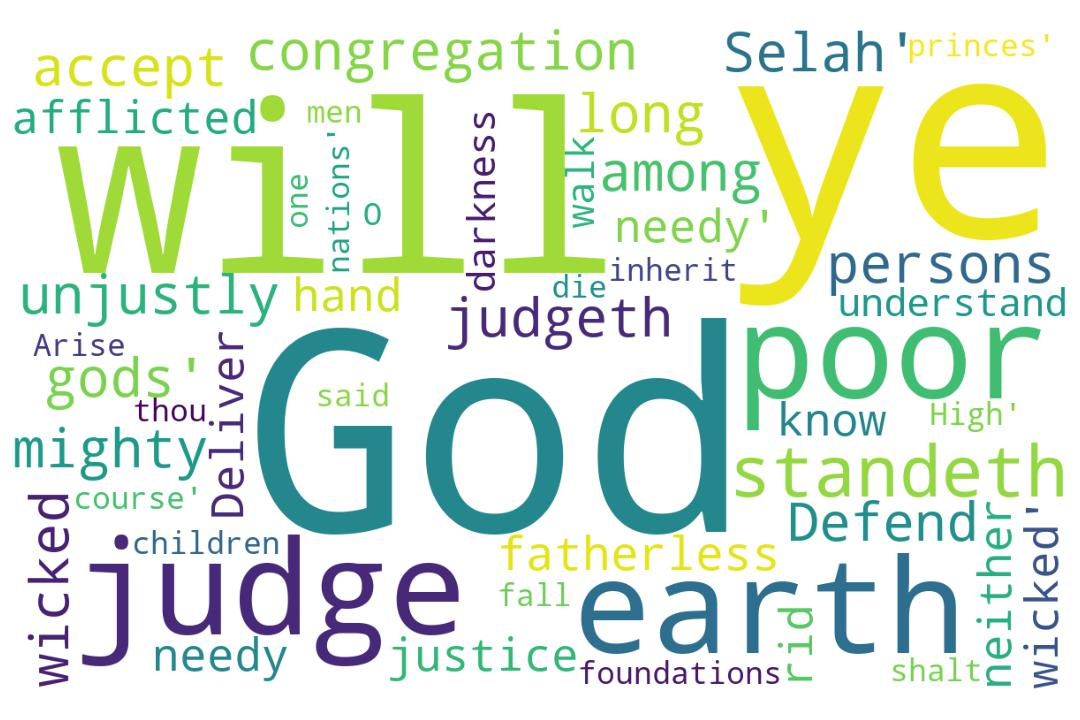
\includegraphics[width=\linewidth]{19OT-Psalms/Psalm82-WordCloud.jpg}
  \caption{Psalm 82 Word Cloud}
  \label{fig:Psalm 82 word Cloud}
\end{figure}

\marginpar{\scriptsize \centering \fcolorbox{bone}{lime}{\textbf{GOD IN CHARGE}}\\ (Psalm 81) \begin{compactenum}[I.][8]
   \item The \textbf{Realm of Leadership} \index[scripture]{Psalms!Psa 082:01}(Psa 82:1) 
    \item The \textbf{Ruin of a Leader} \index[scripture]{Psalms!Psa 082:02}(Psa 82:2) 
    \item The (Proper) \textbf{Regard of a Leader} \index[scripture]{Psalms!Psa 082:03}(Psa 82:3) 
    \item The \textbf{Rebuke of Leaders} \index[scripture]{Psalms!Psa 082:05}(Psa 82:5) 
    \item The \textbf{Reasons for Bad Leaders} \index[scripture]{Psalms!Psa 082:05}(Psa 82:5) 
    \item The \textbf{Return of THE LEADER} \index[scripture]{Psalms!Psa 082:08}(Psa 82:8) 
\end{compactenum}}

\marginpar{\scriptsize \centering \fcolorbox{bone}{yellow}{\textbf{COURT IN SESSION}}\\ (Psalm 81) \begin{compactenum}[I.][8]
   \item The \textbf{Delay} \index[scripture]{Psalms!Psa 082:02}(Psa 82:2) 
   \item The \textbf{Defense} \index[scripture]{Psalms!Psa 082:03}(Psa 82:3) 
   \item The \textbf{Deliverance} \index[scripture]{Psalms!Psa 082:04}(Psa 82:4) 
   \item The \textbf{Darkness} \index[scripture]{Psalms!Psa 082:05}(Psa 82:5) 
   \item The \textbf{Descent} \index[scripture]{Psalms!Psa 082:06}(Psa 82:6) 
   \item The \textbf{Death} \index[scripture]{Psalms!Psa 082:07}(Psa 82:7) 
   \item The \textbf{Disposing} \index[scripture]{Psalms!Psa 082:08}(Psa 82:8) 
\end{compactenum}}


\footnote{\textcolor[rgb]{0.00,0.25,0.00}{\hyperlink{PsalmsTOC}{Return to end of Table of Contents.}}}\footnote{\href{https://audiobible.com/bible/psalms_82.html}{\textcolor[cmyk]{0.99998,1,0,0}{Psalm 82 Audio}}}\textcolor[cmyk]{0.99998,1,0,0}{A Psalm of Asaph.}\\
\\
\textcolor[cmyk]{0.99998,1,0,0}{God standeth in the congregation of the mighty; he judgeth among the gods.}\footnote{\textbf{1 Kings 22:19} - And he said, Hear thou therefore the word of the LORD: I saw the LORD sitting on his throne, and all the host of heaven standing by him on his right hand and on his left.} %\footnote{But here, the spiritual truths give way to Biblical doctrines that are hard to hear, so those “dull of hearing” (Heb. 5:11) are now about to “bomb out” right and left. One will abort, one will miscarry, one will throw in the sponge, and another will move through the Psalm like a drugged sleep walker.\cite{Ruckman1992Psalms}}
[2] \textcolor[cmyk]{0.99998,1,0,0}{How long will ye judge unjustly, and accept the persons of the wicked? Selah.} %\footnote{“The congregation of the mighty” is not any congregation of earthly judges, and  when “he judgeth among the gods,” there is no reference to Israelite judges, any of Aaron’s seed, or anything else. Look at 1 Kings 22:19 for the Holy Spirit’s description of the “congregation of the mighty.” Verse 6 is what destroyed the spiritual sensibilities of Kroll, Duhm, Motyer, Clarke, Lange, Dummelow, Yates, Baethgen, Hengstenberg, and Charles Haddon Spurgeon. You will note that God often makes Charlie pay for his sin of leaning on the corrupt RV, at times, and occasionally aping Westcott and Hort by talking about “better renderings” and “better translations.” There is a price to pay for strutting like a peacock before the Holy Spirit. No man states the truth concerning the power and authority of the King James Bible any better than Spurgeon when he is in his right mind (see the Bible Believers’ Bulletin, September 1990), but alas, “all flesh is grass” and “all have sinned,” etc., so when Charlie tries to impress the stupid apostates of his day—who taught the faculties and staffs of every major Christian college and seminary everything they know—God puts him down as a candidate for blindness at a later date. This is one of those dates. That is the date line. It quickly eliminates every Nicolaitan who was trying to “bring out the intent of the original author” by “translating the Hebrew text in up to date language, so it might communicate to the receptor,” etc. (Interpretation: “He’s got a job that takes a lot of guts: he strings tennis rackets.”) \cite{Ruckman1992Psalms}}
[3] \textcolor[cmyk]{0.99998,1,0,0}{Defend the poor and fatherless: do justice to the afflicted and needy.}
[4] \textcolor[cmyk]{0.99998,1,0,0}{Deliver the poor and needy: rid \emph{them} out of the hand of the wicked.}
[5] \textcolor[cmyk]{0.99998,1,0,0}{They know not, neither will they understand; they walk on in darkness: all the foundations of the earth are out of course.}
[6] \textcolor[cmyk]{0.99998,1,0,0}{I have said, Ye \emph{are} gods; and all of you \emph{are} children of the most High.}
[7] \textcolor[cmyk]{0.99998,1,0,0}{But ye shall die like men, and fall like one of the princes.}\footnote{\textbf{Job 22:15-17} - Hast thou marked the old way which wicked men have trodden? 16 Which were cut down out of time, whose foundation was overflown with a flood: 17 Which said unto God, Depart from us: and what can the Almighty do for them?}\footnote{\textbf{2 Peter 2:4-5} - For if God spared not the angels that sinned, but cast them down to hell, and delivered them into chains of darkness, to be reserved unto judgment; 5 And spared not the old world, but saved Noah the eighth person, a preacher of righteousness, bringing in the flood upon the world of the ungodly;}% \footnote{You do not say: “I have said ye are cats, but ye shall die like cats.” You could say: “I have said ye are dogs, but ye will drown like fishes.” Two things that aren’t the same cannot be equated, so the scholars will have to “fix up” the “men” so they don’t stand in opposition to the “gods.” (That is what Scofield did with Genesis 6:2, so the “daughters of men” could simply be messing around with the “sons of men.” The text said “sons of God.”) This is fourth-grade English. The disjunctive conjunction (“but” vs. 7) shows us that we are not dealing with men; there are no human judges in verses 6–7. The contrast is between someone who might truly be a “god” but he will die like a man—not a “god.” Jamieson, Fausset, and Brown go to bat for every Biblecorrecting Nicolaitan at Liberty University and say that what the Holy Spirit meant to say in verse 7 was “not like any ordinary man.” This solves the problem for the Biblerejecting Fundamentalist who has no grasp of the Scriptures. “I have said you are above ordinary men, but you will die like ordinary men “; i.e., “I will tell you what the Scriptures should have said because as they are written it is impossible for me to understand them.” You see where this type of reasoning winds up? It winds up with “YOU need a different translation because the Holy Bible is impossible for YOU to understand. After all, if I, with my twenty five years of formal education, can’t understand it, how could YOU possibly understand it? Here! Buy this Nutty Imbecile’s Version (NIV). Cash, check, or money order!” See how it’s done? The judges in Genesis 6 corrupted the entire earth with their decisions. They made decisions worse than the ones made by the “nine old men” since 1933. These supernatural “gods” are identified as “gods” in the following places: Genesis 3:5; Exodus 15:11; Psalm 86:8, 95:3, 136:2 (Note THAT one! lmgine thinking those “gods” are Israelite judges!), and Jeremiah 10:11. They are called “the sons of God” in Job 38:7 and Genesis 6:2, so the only way Scofield could remove “children of the most High” from Psalm 82:6 was to pretend that the “gods” were NOT literally “the sons of God.” They were the “sons of Seth”! Had enough of “higher scholarship”? Is this enough from the “recognized scholars” whose “loyalty” to lost pieces of paper is “unquestioned”? Gotta belly full yet, or are you like the little boy who was told “If you eat one more bite, you are going to bust wide open”? He replied, “Please pass the cake and everybody stand back. “ The “gods” have been here before and will be here again. Idols are the mementos that man has used since the flood to commemorate their presence (see Isa. 44:10; Ps. 96:5, 97:7). They came down “in the likeness of men” according to the New Testament (Acts 14:11), so every angel in the Bible appears as a young man (Judg. 13:6; Gen. 19:5; Acts 1:10; Luke 24:4, etc.). Scofield got rid of them again by saying “angels are sexless.” But when he says “ye shall die like men,” he meant they would drown in the flood (2 Pet. 2:4–5; Job 22:15– 17), and so they did. At the time they were judging, Enoch was prophesying the Second Coming of Jesus Christ (see Jude 14). There is a chance that this Psalm may be a pre Deluge Psalm written by Enoch (see remarks under Ps. 90). All the commentators “blew it.” It is evident that once a man begins to mess with the King James text that the Author of Scripture begins to mess with his mind, and pretty soon he cannot get the simplest doctrinal and prophetic truths in order. This statement is proved the moment some blockhead on the faculty at Bob Jones, PCC, Santa Rosa, BBC, or Tennessee Temple tries to cover up his infidelity. We will cite an A 1 example, honed to perfection at Liberty University. Having been told that “all the foundations of the earth are out of course” (vs. 5)—which matches Isaiah 24:19–20—Kroll, of Liberty University, alters them to “the fabric of the nation.” (So help me, Delitzsch and Keil, that is what Lynchburg did with “the Hebrew text.”) ``Yet in the highly poetic language of the Psalm...when the fundamental basis of society, the very principles of morality, are not followed by the judges, the very fabric of the nation is shaken.'' Go sit on a tack. That is modern, “militant Fundamentalist” scholarship in 1992. It is a combination of stupidity, unbelief, arrogance, blindness, and equivocation wrapped up in one neat ball of piety and propagated by men who “don’t like Brother Ruckman’s language.” (I hope to God they don’t, and I hope to God they never will.) \cite{Ruckman1992Psalms}}
[8] \textcolor[cmyk]{0.99998,1,0,0}{Arise, O God, judge the earth: for thou shalt inherit all nations.} %\footnote{There it goes again, in case you missed the “Selah.” But at Liberty University they can’t find EITHER expression in ANY version. Kroll (absolutely spaced out) says that “Arise, O God” is just a “metaphor taken from the common gesture of judges who sit as they hear a case and rise up to pronounce a sentence.” No, that is exactly what the expression didn’t mean one time anywhere in the entire Bible. See Psalm 3:7, 7:6, 9:19, 10:12, 12:5, 17:13, 44:23, 26, 68:1, and 74:22. It wasn’t a “metaphor” one time out of ten. Trust Lynchburg to steal your money as well as your Bible. “For thou shalt inherit all nations” gave you the third clue as to the time, and Kroll still missed it. He had to apply the second half of verse 8 to the Second Advent because he was Premillennial, but being carnal (as well as stupid), he had to limit the first half of the verse to human judges before the Church Age. He, as everyone of his peers, ignored the fact that the ``gods'' will be here in the Tribulation, and they will be reigning not only as kings but as absolute authorities over all judicial matters on earth (Rev. 17:12). They will be in the same position as in Genesis 6:1--6. (Note the word “mighty,” as in Ps. 82:1.) When Christ applied the verse to human judges to prove His own deity (John 10:34--36), He knocked every translator, every reviser, every commentator, and every ``exegete'' slap out of the rink. At no time did God ever say “all of you Israelite judges are children of the most High.” To tell the truth, none of them were; not even the saved ones. The judges in Israel were Levites (Mal. 2:4, 7–8; Deut. 1:16, 21:5), and not one of them was a “child of God.” When John uses the expression (John 11:52), he uses it in a Jewish sense that was not doctrinal. Jesus Christ Himself allows that the Jews of that time were not only NOT the “children of God” (John 8:42--44), they were not even the children of Abraham (John 8:39). That isn’t all: “all the foundations of the earth” (vs. 5) were NOT “out of course” at anytime between Asaph and Paul, and they are not now, nor were they when Moses appointed human judges over Israel (Exodus 18:22, 25; Num. 11:16--17). Someone is “off their trolley” again; they have “one oar in the water.” The problem came from Exodus 22:28. With this and John 10:34, the Bible-correcting apostates took the liberty to throw out the entire context of Psalm 82, since they couldn’t understand it. The context (vss. 1, 5–6, 8) was the Second Advent, and the type was “the days of Noah,” for there the “gods” drowned like “men” (see vs. 7), at least according to 2 Peter 3:6; Jude 6; Job 22:16;  and Revelation 20:13 in the English text. There is nothing like Elizabethan English to make a debacle out of a seminary; especially if it is a bunch of book mad stuffed shirts who think the sun rises and sets on ``plenary, verbally inspired, original autographs.'' (A duck is a bird that walks like he has been riding a horse all day.) Dual application: The judges in Israel could be ``gods'' in the sense that Moses was a “god” to Pharaoh and Aaron (Exod. 7:1). You can be a ``son'' of God because you represent THE Son of God. (The Pope is not shy in the least; he simply applies God’s titles to himself, John 17:11.) The human judges could judge ``the poor and fatherless...the afflicted and needy...the poor and needy,'' so they acted as gods for these people. Final Authority. Get it? You got it yet? Christ merely quotes the passage to show that they have no right to accuse Him of claiming to be something that He is not. He doesn’t tell you one thing about the Psalm or what the Psalm was dealing with. So the Nicolaitans—who have been correcting the Psalms now for ten to three hundred years—can’t find out what is going on. When Christ says that it is written in the Law ``I said, ye are gods,'' the ``ye'' doesn’t have anything to do with anyone to whom He is talking who got ``the word of God.'' The ``ye'' was a reference to angels from Genesis 6 who will show up in the Tribulation. \cite{Ruckman1992Psalms}}



\chapter{Proverb 22}

\begin{figure}
  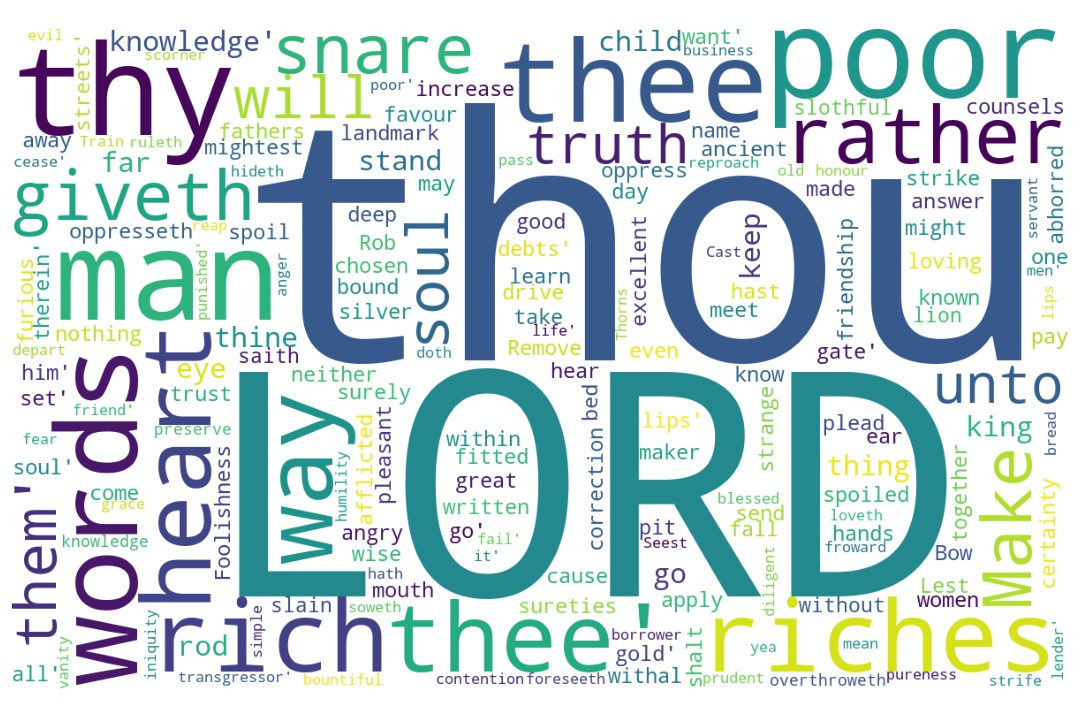
\includegraphics[width=\linewidth]{20OT-Proverbs/Proverb22-WordCloud.jpg}
  \caption{Proverb 22 Word Cloud}
  \label{fig:Proverb 22 word Cloud}
\end{figure}


\marginpar{\scriptsize \centering \fcolorbox{bone}{lime}{\textbf{AN ALL-SEEING GOD}}\\ (Proverb 22:1-29) \begin{compactenum}[I.][8]
    \item \textbf{Are all Around!}(\index[scripture]{Proverbs!Pro 05:21}  \index[scripture]{Proverbs!Pro 15:03}  \index[scripture]{Zechariah!Zch 04:10} (Pro 5:21, Pro 15:3, Zech 4:10)
    \item \textbf{Appraise the Situation} \index[scripture]{1 Kings!1Kng 16:25} \index[scripture]{2 Chronicles!2Chr 14:2}  \index[scripture]{2 Chronicles!2 Chr 21:06}  \index[scripture]{2 Chronicles!2 Chr 29:06} (1Kng 16:25, 2Chr 14:2, 2Chr 21:16, 2Chr 29:6)
    \item \textbf{Are Active} \index[scripture]{Proverbs!Pro 22:12} (Pro 22:12)
    \item \textbf{Approve} \index[scripture]{2 Samuel!2 Sam 15:25} \index[scripture]{Isaiah!Isa 49:05} (2Sam 15:25, Isa 49:5)
    \item \textbf{Are Attentive} (\index[scripture]{Genesis!Gen 6:8}Genesis 06:08, \index[scripture]{2 Chronicles!2 Chr 16:09}2 Chronicles 16:9, \index[scripture]{Psalm!Psa 34:15}Psa 34:15, \index[scripture]{1 Peter!1Pet 03:12}1Pet 3:12)
    \item \textbf{Are Aware} \index[scripture]{Zechariah!Zech 04:10} (Zech 4:10)
    \item \textbf{Analyze} \index[scripture]{Amos!Amo 09:08} (Amos 9:8)
\end{compactenum}}

\marginpar{\scriptsize \centering \fcolorbox{bone}{yellow}{\textbf{SOME ADVICE}}\\ (Proverb 22:1-29) \begin{compactenum}[I.][8]
    \item \textbf{Choice} \index[scripture]{Proverbs!Pro 22:01} (Pro 22:1)
    \item \textbf{Child} \index[scripture]{Proverbs!Pro 22:06}\index[scripture]{Proverbs!Pro 22:15} (Pro 22:6, 15)
    \item \textbf{Contention} \index[scripture]{Proverbs!Pro 22:10} (Pro 22:10)
    \item \textbf{Correction} \index[scripture]{Proverbs!Pro 22:15} (Pro 22:15)
    \item \textbf{Counsels} \index[scripture]{Proverbs!Pro 22:20} (Pro 22:20)
    \item \textbf{Certainty} \index[scripture]{Proverbs!Pro 22:21} (Pro 22:21)
    \item \textbf{Cause} \index[scripture]{Proverbs!Pro 22:23} (Pro 22:23)
\end{compactenum}}

\footnote{\textcolor[cmyk]{0.99998,1,0,0}{\hyperlink{TOC}{Return to end of Table of Contents.}}}\footnote{\href{https://audiobible.com/bible/proverbs_22.html}{\textcolor[cmyk]{0.99998,1,0,0}{Proverbs Audio}}}\textcolor[cmyk]{0.99998,1,0,0}{A \emph{good} name \emph{is} rather to be \fcolorbox{bone}{lime}{chosen} than great riches, \emph{and} loving favour rather than silver and gold.}
[2] \textcolor[cmyk]{0.99998,1,0,0}{The rich and poor meet together: the LORD \emph{is} the maker of them all.}
[3] \textcolor[cmyk]{0.99998,1,0,0}{A prudent \emph{man} foreseeth the evil, and hideth himself: but the simple pass on, and are punished.}
[4] \textcolor[cmyk]{0.99998,1,0,0}{By humility \emph{and} the fear of the LORD \emph{are} riches, and honour, and life.}
[5] \textcolor[cmyk]{0.99998,1,0,0}{Thorns \emph{and} snares \emph{are} in the way of the froward: he that doth keep his soul shall be far from them.}
[6] \textcolor[cmyk]{0.99998,1,0,0}{Train up a \fcolorbox{bone}{lime}{child} in the way he should go: and when he is old, he will not depart from it.}
[7] \textcolor[cmyk]{0.99998,1,0,0}{The rich ruleth over the poor, and the borrower \emph{is} servant to the lender.}
[8] \textcolor[cmyk]{0.99998,1,0,0}{He that soweth iniquity shall reap vanity: and the rod of his anger shall fail.}
[9] \textcolor[cmyk]{0.99998,1,0,0}{He that hath a bountiful eye shall be blessed; for he giveth of his bread to the poor.}\footnote{See Proverbs 21:26 and 14:21. The Roman Vulgate and Alexandrian Septuagint add about eleven to fifteen words not found in the Bible and prove, again, that “Western” and “Alexandrian” manuscripts for the New Testament have the same type of writers, admirers, “preservers,” and believers. For 22:9, the LXX has: ``He that has pity on the poor shall himself be maintained; for he has given of his own bread to the poor. He that gives liberally secures victory an honour; but he takes away the life of them that posses.''}\footnote{\textbf{Proverb 14:21} - He that despiseth his neighbour sinneth: but he that hath mercy on the poor, happy is he.}\footnote{\textbf{Proverb 21:26} - He coveteth greedily all the day long: but the righteous giveth and spareth not.}
[10] \textcolor[cmyk]{0.99998,1,0,0}{Cast out the scorner, and \fcolorbox{bone}{lime}{contention} shall go out; yea, strife and reproach shall cease.}
[11] \textcolor[cmyk]{0.99998,1,0,0}{He that loveth pureness of heart, \emph{for} the grace of his lips the king \emph{shall} \emph{be} his friend.}\footnote{The proverb is clear; especially so in the light of Matthew 5:8 and 2 Samuel 22:27 (see further comment under 21:8). Since God is pure (Hab. 1:13) and the word of God is pure (Psa. 119:140), the “king” (see comments under 20:2, 8 and 21:1) will accept the “pure in heart.” “For the grace of his lips” implies that the pure in heart speaks out of the abundance of his heart (Matt. 5:8). These “lips” are found again in Proverbs 8:6, 10:13, 10:21, 32, 12:19, 14:3, 15:7, and 16:10.}
[12] \textcolor[cmyk]{0.99998,1,0,0}{The eyes of the LORD preserve knowledge, and he overthroweth the words of the transgressor.}
[13] \textcolor[cmyk]{0.99998,1,0,0}{The slothful \emph{man} saith, \emph{There} \emph{is} a lion without, I shall be slain in the streets.}
[14] \textcolor[cmyk]{0.99998,1,0,0}{The mouth of strange women \emph{is} a deep pit: he that is abhorred of the LORD shall fall therein.}
[15] \textcolor[cmyk]{0.99998,1,0,0}{Foolishness \emph{is} bound in the heart of a \fcolorbox{bone}{lime}{child}; \emph{but} the rod of \fcolorbox{bone}{lime}{correction} shall drive it far from him.}
[16] \textcolor[cmyk]{0.99998,1,0,0}{He that oppresseth the poor to increase his \emph{riches,} \emph{and} he that giveth to the rich, \emph{shall} surely \emph{come} to want.}
[17] \textcolor[cmyk]{0.99998,1,0,0}{Bow down thine ear, and hear the words of the wise, and apply thine heart unto my knowledge.}
[18] \textcolor[cmyk]{0.99998,1,0,0}{For \emph{it} \emph{is} a pleasant thing if thou keep them within thee; they shall withal be fitted in thy lips.}
[19] \textcolor[cmyk]{0.99998,1,0,0}{That thy trust may be in the LORD, I have made known to thee this day, even to thee.}
[20] \textcolor[cmyk]{0.99998,1,0,0}{Have not I written to thee excellent things in \fcolorbox{bone}{lime}{counsels} and knowledge,}
[21] \textcolor[cmyk]{0.99998,1,0,0}{That I might make thee know the \fcolorbox{bone}{lime}{certainty} of the words of truth; that thou mightest answer the words of truth to them that send unto thee?}
[22] \textcolor[cmyk]{0.99998,1,0,0}{Rob not the poor, because he \emph{is} poor: neither oppress the afflicted in the gate:}
[23] \textcolor[cmyk]{0.99998,1,0,0}{For the LORD will plead their \fcolorbox{bone}{lime}{cause}, and spoil the soul of those that spoiled them.}
[24] \textcolor[cmyk]{0.99998,1,0,0}{Make no friendship with an angry man; and with a furious man thou shalt not go:}
[25] \textcolor[cmyk]{0.99998,1,0,0}{Lest thou learn his ways, and get a snare to thy soul.}
[26] \textcolor[cmyk]{0.99998,1,0,0}{Be not thou \emph{one} of them that strike hands, \emph{or} of them that are sureties for debts.}
[27] \textcolor[cmyk]{0.99998,1,0,0}{If thou hast nothing to pay, why should he take away thy bed from under thee?}
[28] \textcolor[cmyk]{0.99998,1,0,0}{Remove not the ancient landmark, which thy fathers have set.}\footnote{\textbf{Deuteronomy 19:14} - Thou shalt not remove thy neighbour’s landmark, which they of old time have set in thine inheritance, which thou shalt inherit in the land that the LORD thy God giveth thee to possess it.}\footnote{\textbf{Deuteronomy 27:17} - Cursed be he that removeth his neighbour’s landmark. And all the people shall say, Amen.}\footnote{\textbf{Proverb 23:10} - Remove not the old landmark; and enter not into the fields of the fatherless:}
[29] \textcolor[cmyk]{0.99998,1,0,0}{Seest thou a man diligent in his business? he shall stand before kings; he shall not stand before mean \emph{men}.}\footnote{\textbf{Proverb 21:5} - he thoughts of the diligent tend only to plenteousness; but of every one that is hasty only to want.}\footnote{\textbf{Proverb 27:23} - Be thou diligent to know the state of thy flocks, and look well to thy herds.}\footnote{\textbf{2 Peter 3:14} - Wherefore, beloved, seeing that ye look for such things, be diligent that ye may be found of him in peace, without spot, and blameless.}




\end{document}

